\documentclass[10pt,tgadventor, onlymath]{beamer}

\usepackage{graphicx,amsmath,amssymb,tikz,psfrag,neuralnetwork}

\input defs.tex
\graphicspath{ {./figures/} }

%% formatting

\mode<presentation>
{
\usetheme{default}
\usecolortheme{seahorse}
}
\setbeamertemplate{navigation symbols}{}
\usecolortheme[rgb={0.03,0.28,0.59}]{structure}
\setbeamertemplate{itemize subitem}{--}
\setbeamertemplate{frametitle} {
	\begin{center}
	  {\large\bf \insertframetitle}
	\end{center}
}

\newcommand\footlineon{
  \setbeamertemplate{footline} {
    \begin{beamercolorbox}[ht=2.5ex,dp=1.125ex,leftskip=.8cm,rightskip=.6cm]{structure}
      \footnotesize \insertsection
      \hfill
      {\insertframenumber}
    \end{beamercolorbox}
    \vskip 0.45cm
  }
}
\footlineon

\AtBeginSection[] 
{ 
	\begin{frame}<beamer> 
		\frametitle{Outline} 
		\tableofcontents[currentsection,currentsubsection] 
	\end{frame} 
} 


\tikzstyle{state}=[shape=circle,draw=blue!30,fill=blue!10]
\tikzstyle{observation}=[shape=rectangle,draw=orange!30,fill=orange!10]
\tikzstyle{lightedge}=[<-, dashed]
\tikzstyle{mainstate}=[state, thick]
\tikzstyle{mainedge}=[<-, thick]
\tikzstyle{block} = [draw,rectangle,thick,minimum height=2em,minimum width=2em]
\tikzstyle{sum} = [draw,circle,inner sep=0mm,minimum size=2mm]
\tikzstyle{connector} = [->,thick]
\tikzstyle{line} = [thick]
\tikzstyle{branch} = [circle,inner sep=0pt,minimum size=1mm,fill=black,draw=black]
\tikzstyle{guide} = []
\tikzstyle{snakeline} = [connector, decorate, decoration={pre length=0.2cm,
                         post length=0.2cm, snake, amplitude=.4mm,
                         segment length=2mm},thick, magenta, ->]



%% begin presentation

\title{\large \bfseries Neural Network Metrics for Viterbi Decoding in Molecular Communication Channels}

\author{Peter Hartig\\[3ex]
}

\date{\today}

\begin{document}

\frame{
\thispagestyle{empty}
\titlepage
}

\section{Background}

\begin{frame}<0>
\frametitle{Viterbi Setup}
	Probability of transmitted symbol sequence given the received signal
	\begin{equation}
		Pr(\mathbf{\mathrm{transmit \;signal}\;= x}|\mathbf{\mathrm{received \;signal}\; = y})
	\end{equation}
	For channels without inter-symbol interference
	\begin{equation}
		\prod_{\mathrm{i=1}}^{\mathrm{n}}pr(x_{\mathrm{i}}|y_{\mathrm{i}}) 
	\end{equation}
	Using Baye's rule
	\begin{equation}
		Pr(x|y) = \frac{Pr(y|x) Pr(x)}{Pr(y)}
	\end{equation}
	With equiprobable transmit symbols
	\begin{equation}
		Pr(y|x) = Pr(x|y) Pr(y)
	\end{equation}

\end{frame}

\begin{frame}
\frametitle{Viterbi Setup}
Maximum Likelihood sequence decoding can be formalized as 
	
	\begin{equation}
	\begin{array}{ll}
		\underset{\mathbf{x}}{\mathrm{maximize}} 	&	Pr(\mathbf{y}|\mathbf{x})
		
		\\
		\underset{\mathbf{x}}{\mathrm{maximize}} &\prod_{\mathrm{i=1}}^{\mathrm{N}}Pr(y_{\mathrm{i}}|\mathbf{x})
		\\ 
		\\
		\underset{\mathbf{x}}{\mathrm{minimize}} &\sum_{\mathrm{i=1}}^{\mathrm{N}} -log(Pr(y_{\mathrm{i}}|\mathbf{x})) 
	\end{array}
	\end{equation}
	\bigskip
	\\
	\begin{center}
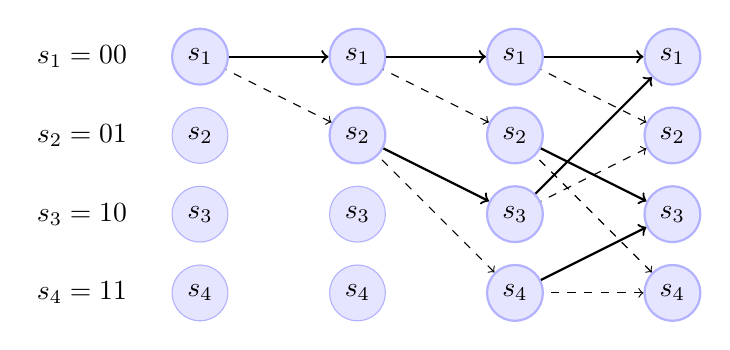
\begin{tikzpicture}[]
% 1st column
\node               at (-1.5,5) {$s_1=00$};
\node               at (-1.5,4) {$s_2=01$};
\node               at (-1.5,3) {$s_3=10$};
\node               at (-1.5,2) {$s_4=11$};
\node[mainstate] (s1_1) at (0,5) {$s_1$};
\node[state] (s2_1) at (0,4) {$s_2$};
\node[state] (s3_1) at (0,3) {$s_3$};
\node[state] (s4_1) at (0,2) {$s_4$};
%\node at (0,1) {Node1};
% 2nd column
\node[mainstate] (s1_2) at (2,5) {$s_1$}
    edge[mainedge] (s1_1);
\node[mainstate] (s2_2) at (2,4) {$s_2$}
     edge[lightedge] (s1_1);

\node[state] (s3_2) at (2,3) {$s_3$};

\node[state] (s4_2) at (2,2) {$s_4$};

%\node at (2,1) {Node2};
% 3rd column
%\node               at (4,6) {$t=2$};
\node[mainstate] (s1_3) at (4,5) {$s_1$}
    edge[mainedge]  (s1_2);

\node[mainstate] (s2_3) at (4,4) {$s_2$}
    edge[lightedge] (s1_2);

\node[mainstate] (s3_3) at (4,3) {$s_3$}
    edge[mainedge] (s2_2);    
\node[mainstate] (s4_3) at (4,2) {$s_4$}
    edge[lightedge] (s2_2);
%\node at (4,1) {Node3};
% 4th column
%\node               at (6,6) {$t=3$};
\node[mainstate] (s1_4) at (6,5) {$s_1$}
    edge[mainedge]  (s1_3)
    edge[mainedge]  (s3_3);
\node[mainstate] (s2_4) at (6,4) {$s_2$}
    edge[lightedge] (s1_3)
    edge[lightedge] (s3_3);
\node[mainstate] (s3_4) at (6,3) {$s_3$}
    edge[mainedge] (s2_3)
    edge[mainedge] (s4_3);
\node[mainstate] (s4_4) at (6,2) {$s_4$}
    edge[lightedge] (s2_3)
    edge[lightedge] (s4_3);
%\node at (6,1) {Node4};

\end{tikzpicture}
	\end{center}

\end{frame}


\begin{frame}
\frametitle{Viterbi Setup Continued}

Each state change is decided by the metric $ Pr(y_{\mathrm{i}}|\mathbf{x})$. In a linear channel with length $l$ impulse response , this metric becomes 
$ Pr(y_{\mathrm{i}}|\mathbf{x}_{\mathrm{i-l}}^{\mathrm{i}})$.
	
	\bigskip

	\begin{center}
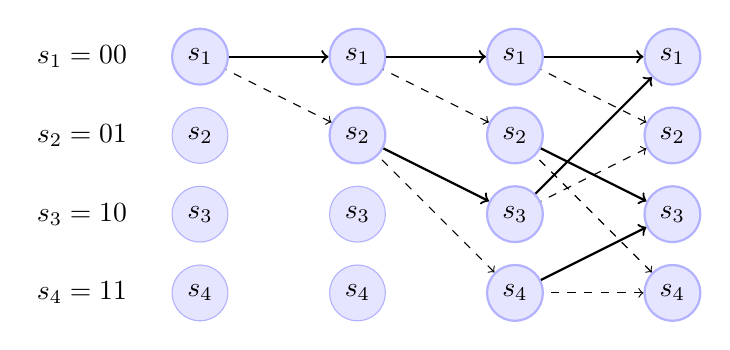
\begin{tikzpicture}[]
% 1st column
\node               at (-1.5,5) {$s_1=00$};
\node               at (-1.5,4) {$s_2=01$};
\node               at (-1.5,3) {$s_3=10$};
\node               at (-1.5,2) {$s_4=11$};
\node[mainstate] (s1_1) at (0,5) {$s_1$};
\node[state] (s2_1) at (0,4) {$s_2$};
\node[state] (s3_1) at (0,3) {$s_3$};
\node[state] (s4_1) at (0,2) {$s_4$};
%\node at (0,1) {Node1};
% 2nd column
\node[mainstate] (s1_2) at (2,5) {$s_1$}
    edge[mainedge] (s1_1);
\node[mainstate] (s2_2) at (2,4) {$s_2$}
     edge[lightedge] (s1_1);

\node[state] (s3_2) at (2,3) {$s_3$};

\node[state] (s4_2) at (2,2) {$s_4$};

%\node at (2,1) {Node2};
% 3rd column
%\node               at (4,6) {$t=2$};
\node[mainstate] (s1_3) at (4,5) {$s_1$}
    edge[mainedge]  (s1_2);

\node[mainstate] (s2_3) at (4,4) {$s_2$}
    edge[lightedge] (s1_2);

\node[mainstate] (s3_3) at (4,3) {$s_3$}
    edge[mainedge] (s2_2);    
\node[mainstate] (s4_3) at (4,2) {$s_4$}
    edge[lightedge] (s2_2);
%\node at (4,1) {Node3};
% 4th column
%\node               at (6,6) {$t=3$};
\node[mainstate] (s1_4) at (6,5) {$s_1$}
    edge[mainedge]  (s1_3)
    edge[mainedge]  (s3_3);
\node[mainstate] (s2_4) at (6,4) {$s_2$}
    edge[lightedge] (s1_3)
    edge[lightedge] (s3_3);
\node[mainstate] (s3_4) at (6,3) {$s_3$}
    edge[mainedge] (s2_3)
    edge[mainedge] (s4_3);
\node[mainstate] (s4_4) at (6,2) {$s_4$}
    edge[lightedge] (s2_3)
    edge[lightedge] (s4_3);
%\node at (6,1) {Node4};

\end{tikzpicture}
	\end{center}
			Example with channel impulse response length 2 and constellation size 2.

\end{frame}

\begin{frame}
	\frametitle{Incorporating Neural Net into Viterbi Decoding}
	\begin{block}{Problem 1}
	Viterbi algorithm requires the distribution $ Pr(y_{\mathrm{i}}|\mathbf{x}_{\mathrm{i-l}}
	^{\mathrm{i}})$.
	\begin{itemize}
			\item \begin{block}{Solution}
Have a neural network learn $ Pr(y_{\mathrm{i}}|\mathbf{x}_{\mathrm{i-l}}^{\mathrm{i}})$.
		\end{block}
\end{itemize}		
	\end{block}


		\begin{block}{Problem 2}
Generating training data $ Pr(y_{\mathrm{i}}|\mathbf{x}_{\mathrm{i-l}}^{\mathrm{i}})$ requires knowledge of the channel and its (current) parameters.
\begin{itemize}
\item 
		\begin{block}{Solution}
		Decompose $ Pr(y_{\mathrm{i}}|\mathbf{x}_{\mathrm{i-l}}^{\mathrm{i}})$ into 
		\begin{gather}
		Pr(y_{\mathrm{i}}|\mathbf{x}_{\mathrm{i-l}}^{\mathrm{i}}) = \frac{Pr(\mathbf{x}_{\mathrm{i-l}}^{\mathrm{i}}|y_{\mathrm{i}})Pr(y_{\mathrm{i}})}{Pr(\mathbf{x}_{\mathrm{i-l}}^{\mathrm{i}})}
		\end{gather}
		\end{block}
\end{itemize}
		\end{block}.


\end{frame}


\begin{frame}[fragile]
	\frametitle{Metrics for $Pr(x_{\mathrm{i-l}}^{\mathrm{i}}|y_{\mathrm{i}})$}
	\begin{figure}
		\begin{neuralnetwork}[height=4, nodespacing=10mm, layerspacing=15mm]
		\newcommand{\x}[2]{$x_#2$}
		\newcommand{\y}[2]{$\hat{y}_#2$}
		\newcommand{\hfirst}[2]{\small $h^{(1)}_#2$}
		\newcommand{\hsecond}[2]{\small $h^{(2)}_#2$}
		\newcommand{\hthird}[2]{\small $h^{(3)}_#2$}
		\newcommand{\hfourth}[2]{\small $h^{(4)}_#2$}
		\inputlayer[count=1, bias=false, title=Received\\, text=\x]
		\hiddenlayer[count=2, bias=false, title=\\, text=\hthird] \linklayers
		\hiddenlayer[count=3, bias=false, title=\\, text=\hfourth] \linklayers
		\outputlayer[count=4, title=States\\, text=\x] \linklayers
	    \end{neuralnetwork}
	\end{figure}
	%We can take the output of an intermediate layer after training as use it as the input features for a
	%classification neural network.
\end{frame}


\begin{frame}
	\frametitle{Metrics for $Pr(y_{\mathrm{i}})$}
	Gaussian Mixture Model using  Expectation-Maximization algorithm
		\includegraphics[width=\textwidth,height=7cm]{em_figure}
\end{frame}



\section{Initial Results}

\begin{frame}
\frametitle{Detection Performance}
\begin{columns}
\begin{column}{0.5\linewidth}
	Without ISI

	\includegraphics[width=\textwidth]{no_isi}
\end{column}
\begin{column}{0.5\linewidth}
	With ISI

	\includegraphics[width=\textwidth]{without_mm}

\end{column}
\end{columns}
\end{frame}

\begin{frame}
\frametitle{Detection Performance}
	Reduced Training data (100 vs. 1000 symbols)
	\includegraphics[width=\textwidth,height = 7cm]{low_training_data}
\end{frame}


\begin{frame}
\frametitle{Next Steps}
\begin{itemize}
\item Improve decoding performance with neural net.
\item Apply to a sampled molecular communications channel.
\begin{itemize}
\item Estimate matched filter
\end{itemize}
\item Generate training data for molecular communications channel and test "transfer learning" to real data.
\end{itemize}
\end{frame}

\begin{frame}
  \centering \Large
  \emph{Thank You.}
  \\
	\bigskip
    \centering \Large
  \emph{Questions or Comments?}

\end{frame}





\end{document}
